\scanpage{103}
\mspage{10}

\deleted{$e_0\mathbin{-}e_1$}

\figure{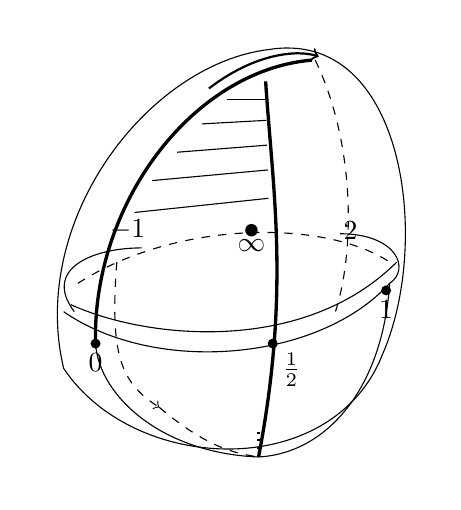
\begin{tikzpicture}[x=1cm,y=1cm,scale=.9]
\draw (0,0) .. controls (-.5,2.1) and (1.2,4.3) .. (2.9,4.5)
 .. controls (4.8,4.8) and (5.2,1.8) .. (4.5,.2)
 .. controls (3.8,-1.6) and (1,-1.5) .. (0,0);
\draw (.1,.9) .. controls (1.2,.4) and (3.4,.2) .. (4.7,1.5);
\draw (0,.8) .. controls (1.3,-.1) and (3.6,.1) .. (4.6,1.2);
\draw[dashed] (.2,1.2) .. controls (1.6,2.1) and (3.7,2.1) .. (4.6,1.5);
\draw (.15,.8) .. controls (-.3,1.4) and (.4,1.7) .. (1.1,1.7);
\draw (3.9,1.9) .. controls (4.7,1.9) and (4.9,1.4) .. (4.6,1.2);
\draw[very thick] (.45,.35) .. controls (.4,2.3) and (1.8,4.2) .. (3.5,4.35);
\draw[thick,->] (2.05,3.95) .. controls (2.7,4.45) and (3.3,4.5) .. (3.6,4.4);
\draw[very thick] (2.85,4.05) .. controls (2.95,2.5) and (3.2,1.1) .. (2.75,-1.25);
\draw[dotted,thick] (2.75,-1.25)--(2.75,-.85);
\draw[dashed,->] (.75,1.5) .. controls (.65,.2) and (.8,-.2) .. (1.35,-.55);
\draw[dashed] (1.35,-.55) .. controls (2,-1.1) and (2.4,-1.2) .. (2.75,-1.25);
\draw[dashed] (3.55,4.35) .. controls (4.15,3.1) and (4.1,1.5) .. (3.8,.7);
\draw (4.6,1.2) .. controls (4.5,-.3) and (3.7,-1.2) .. (2.75,-1.25);
\draw (.45,.35) .. controls (.5,-.4) and (1.4,-1.2) .. (2.75,-1.25);
\draw (1.0,2.2)--(2.89,2.4);
\draw (1.25,2.65)--(2.88,2.8);
\draw (1.6,3.05)--(2.87,3.15);
\draw (1.95,3.45)--(2.86,3.5);
\draw (2.3,3.8)--(2.86,3.8);
\fill (.45,.35) circle(2pt) node[below] {$0$};
\fill (2.95,.35) circle(2pt) node[below right] {$\frac12$};
\fill (4.55,1.1) circle(2pt) node[below] {$1$};
\fill (2.65,1.95) circle(2.5pt) node[below] {$\infty$};
\node at (.9,1.95) {$-1$}; \node at (4.05,1.95) {$2$};
\end{tikzpicture}}

\diagram{\begin{array}{cc}
\begin{tikzcd}[ampersand replacement=\&,row sep=small]
e_0\arrow[r,maps to]\&e_{\unsure{0|\rho}}\\
e_1\arrow[r,maps to]\&e_1-e_0
\end{tikzcd}
&
\left|\begin{tikzcd}[ampersand replacement=\&,row sep=small]
e_0\arrow[r]\&e_1\\
e_1\arrow[r]\&-e_0
\end{tikzcd}\right.
\end{array}}

\deleted{$\unsure{B|R}$}
\diagram{\begin{tikzcd}[ampersand replacement=\&,row sep=small]
e_0\arrow[r]\&e_0+e_1\\
e_1\arrow[r,maps to]\&-e_0
\end{tikzcd}}

\[
\begin{pmatrix}1&\lambda\\0&\unsure{\phi|1}\end{pmatrix}
\qquad
\begin{pmatrix}\unsure{\zeta|\lambda}&0\\0&\zeta^*\end{pmatrix}
\]

\deleted{$(\unsure{\varphi}\,\unsure{\varphi}\mathbin{-}\unsure{\tau}$}

\[
\det(u-\lambda\mathrm{id})
=\det\begin{pmatrix}1-\lambda&-1\\1&-\lambda\end{pmatrix}
\underset{\deleted{\unsure{z}}}{=}\lambda^2-\lambda+1
\]
racines sont racines primitives \unsure{6ièmes} de 1

\figure{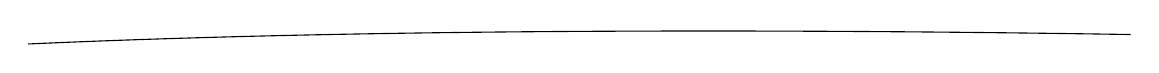
\begin{tikzpicture}[x=1cm,y=1cm]\draw (0,0) .. controls (4,.18) and (9,.2) .. (14,.12);\end{tikzpicture}}

\[
l_0\quad l_{1/2}\quad l_1\quad l_\infty
\qquad/\qquad
\dot{\sigma}_\infty,\ \unsure{\widetilde{\tau}|\widehat{\tau}},\ \sigma_\infty\tau
\]
\[
\boxed{l_\infty l_1 l_{1/2}l_0=1}
\]
\[
z\longmapsto1-z
\]
\diagram{\begin{tikzcd}[ampersand replacement=\&,row sep=small]
g:\ \mathbb P^1\arrow[r]\&\mathbb P^1\\
\infty\arrow[r,maps to]\&\infty\\
\frac12\arrow[r,maps to]\&0\\
0,1\arrow[r,maps to]\&1
\end{tikzcd}}

\[
g(z)=(2z-1)^2
\qquad
g(1-z)=(1-2z)^2.
\]
\[
(2z-\unsure{\tfrac12|\tfrac14})^2
\]

\diagram{\begin{tikzcd}[ampersand replacement=\&,row sep=small]
l_{\unsure{0|\infty}}\arrow[r,maps to]\&-1\\
l_1\arrow[r,maps to]\&+1\\
l_\infty\arrow[r,maps to,no head]\&-1
\end{tikzcd}}

\margin{102}
